\section{Principio di funzionamento}
\subsection{L'apparato circolatorio}
L'apparato circolatorio è fondamentale per la sopravvivenza di tutte le cellule del corpo umano. Il suo compito è quello di provvedere ai bisogni dei tessuti, mantenendo un ambiente adeguato alla sopravvivenza delle cellule che li compongono (omeostasi)\cite{Cevese2002}. 
L'apparato cardiocircolatorio è composto da tre elementi fondamentali:
\begin{enumerate}
\item il sangue, una sospensione di cellule e frazioni cellulari (globuli rossi, globuli bianchi e piastrine) in un liquido acquoso (plasma), contenente proteine e elettroliti;
\item il cuore, un muscolo che, agendo come una pompa, fornisce al sangue la pressione necessaria per poter circolare in tutto il corpo;
\item i vasi sanguigni, un circuito di condotti che permettono al sangue di scorrere lungo tutto il corpo.
\end{enumerate}
Grazie a questo apparato, è possibile trasportare gas respiratori (anidride carbonica e ossigeno), sostanze nutritive (glucosio, aminoacidi, acidi grassi) e messaggi chimici (ormoni) verso tutte le cellule dei tessuti. Inoltre, vengono raccolte e eliminate tutte le sostanze di scarto, prodotte  dalle reazioni chimiche che avvengono nelle cellule. La loro eliminazione è affidata a organi specializzati, come i reni e il fegato, che agiscono come dei filtri, oppure ai polmoni, che permettono lo scambio gassoso, eliminando l'anidride carbonica e assimilando l'ossigeno. Il sangue è anche un elemento che permette la termoregolazione all'interno degli esseri viventi: variando il flusso nei tessuti più esterni è possibile controllare la dispersione del calore corporeo con l'ambiente esterno. Il volume e il flusso di sangue nei tessuti viene controllato dall'azione coordinata di cuore e vasi sanguigni, che insieme permettono di regolarne l'apporto.

All'interno del sistema circolatorio è possibile identificare diverse tipologie di vasi che si differenziano per struttura e funzione. Si suddividono in: arterie, arteriole, capillari, venule e vene. Ciononostante, tutte le pareti vasali sono costituite, in proporzioni variabili, da: endotelio, fibre collagene, fibre elastiche e fibre muscolari lisce. 
Le \textit{arterie} hanno il compito di trasportare il sangue ad alta pressione dal cuore verso i tessuti. A tal fine, analizzando la loro struttura, si possono notare delle pareti vascolari molto resistenti e flessibili. L'arteria principale è l'aorta, che si estende dal ventricolo sinistro  fino alla biforcazione iliaca e permette al sangue arterioso (ricco di ossigeno) di raggiungere i vasi arteriosi di calibro inferiore.
Il sistema arterioso termina con le \textit{arteriole}, che regolano la quantità di sangue immessa nei capillari. Per questo motivo, presentano forti pareti muscolari, che ne permettono la dilatazione o la costrizione.
I \textit{capillari} presentano invece pareti molto sottili e porose, che li rendono permeabili all'acqua e ad alcune molecole. Infatti, a loro è affidato il compito di permettere lo scambio di fluidi e sostanze tra il sangue e il liquido interstiziale delle cellule. 
Infine, le \textit{venule} raccolgono il sangue dei capillari e gradualmente si fondono nelle vene, condotti più larghi, adibiti al trasporto del sangue verso il cuore. In aggiunta, esse costituiscono un'importante riserva ematica, contenendone circa il 65\%. Le vene si differenziano dalle arterie per avere pareti più sottili, in quanto adibite al trasporto di sangue con una minore pressione \cite{Armentano2019}. In aggiunta, alcune vene presenti soprattutto nelle gambe, presentano delle valvole a \textit{nido di rondine}, che impediscono reflusso del sangue. 

Analizzando la complessa rete vascolare, è possibile identificare due sotto-circuiti principali \Fig~\ref{fig:SistemaCircolatorio}:
\begin{figure}[h]
	\centering
	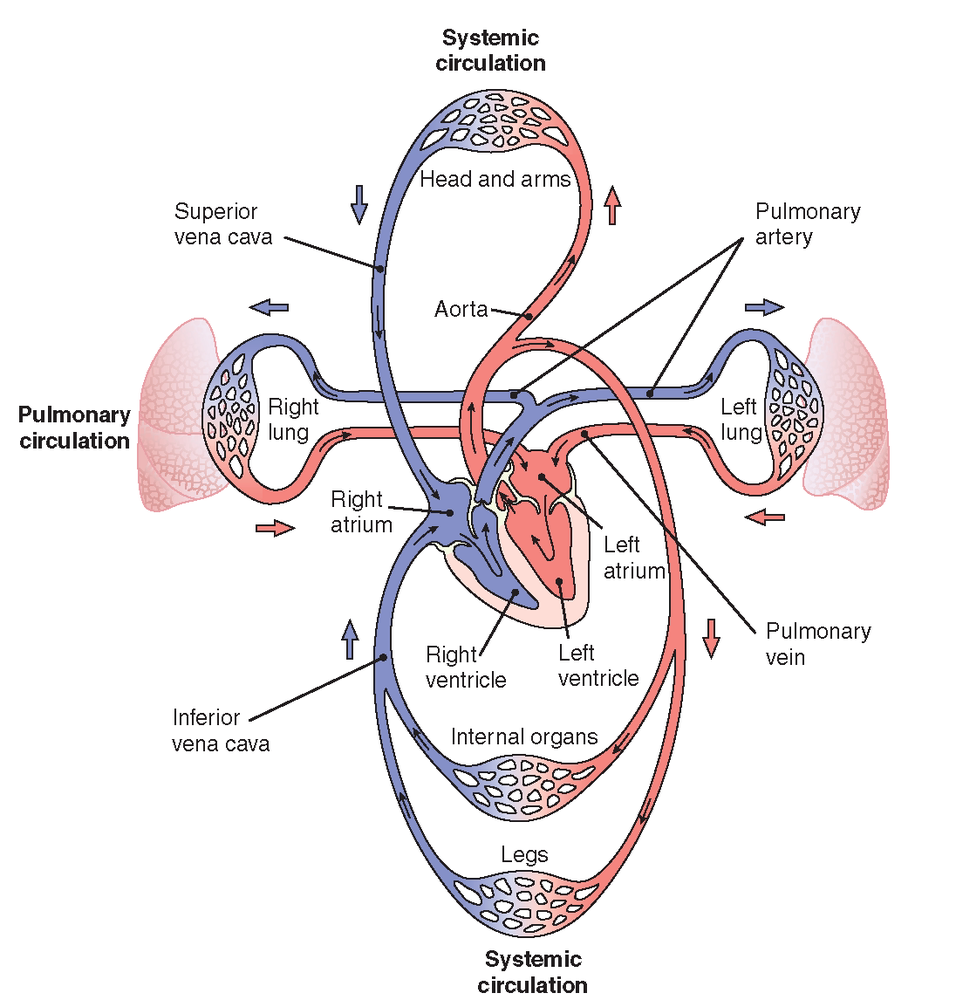
\includegraphics[width=0.7\linewidth]{ImageFiles/Fotopletismografia/SistemaCircolatorio}
	\caption{Rappresentazione del sistema circolatorio.}
	\label{fig:SistemaCircolatorio}
\end{figure}
\begin{itemize}
	\item la \textit{circolazione polmonare}, o piccola circolazione, che include i vasi che dal ventricolo destro del cuore si capillarizza a livello degli alveoli polmonari e ritorna al cuore nell'atrio sinistro tramite le \textit{vene polmonari};
	\item la \textit{circolazione sistemica}, o grande circolazione, che permette al sangue di scorrere dal ventricolo sinistro all'interno dell'\textit{aorta} per poi raggiungere tutto il corpo e ritornare, grazie alla \textit{vena cava}, all'atrio destro.
\end{itemize}
Tuttavia, la distinzione nei due circuiti è puramente concettuale \todo{non mi piace molto} e, in realtà, i due sono strettamente interdipendenti \cite{Cutfield1983}. In effetti, il sangue deossigenato, proveniente \todo{cfr. fonte: https://www.kenhub.com/en/library/anatomy/circulatory-system} dalla circolazione sistemica, ritorna all'atrio destro attraverso la vena cava superiore e inferiore. Durante la fase di \textit{diastole}, scorre nel ventricolo destro attraverso la \textit{valvola tricuspide} e successivamente, grazie alla contrazione del ventricolo (fase di \textit{diastole}), viene spinto nell'arteria polmonare destra e sinistra, che portano il sangue ai polmoni. Grazie ai capillari polmonari avviene il processo di \textit{ematosi}, durante il quale il sangue assimila ossigeno e cede anidride carbonica. Le vene polmonari raccolgono il sangue appena ossigenato e lo conducono nell'atrio sinistro. A questo punto, si ha il punto di passaggio dalla circolazione polmonare alla circolazione sistemica. Dall'atrio destro, attraverso la \textit{valvola bicuspide}, il sangue procede verso il ventricolo sinistro nella la fase di diastole. In seguito, la sistole costringe il sangue nell'aorta che diramandosi fino ai capillari permette la perfusione in tutti i tessuti. Infine, il sangue viene riportato all'atrio destro attraverso le vene cave superiore e inferiore. Il ciclo può ora ripartire. 

\subsection{La circolazione: Pressione, Flusso e Resistenza}
\todo{inserire parte sulla velocità differente del sangue nelle varie parti del corpo?}
Il sangue è assimilabile a un fluido e, come tale, è in grado di scorrere solamente se è presente un \textit{gradiente di pressione} nei vasi sanguigni. Più precisamente, liquidi e gas fluisco da regioni a maggiore pressione verso regioni a minore pressione. Negli esseri umani, il gradiente è mantenuto grazie alle contrazioni del cuore. Infatti, il sangue esce dal cuore con una pressione elevata e fluisce nei circuiti chiusi dei vasi sanguigni dove la pressione diminuisce progressivamente.\cite{SilverthornDeeUnglaub2020Fu:u}.
Come mostrato nella figura \Fig~\ref{fig:PressioneSangue}, all'interno dell'aorta la pressione è mediamente alta e pari a circa 100 mm Hg. Più precisamente, la pressione risulta essere pulsante con dei picchi di 120 mm Hg (\textit{pressione sistolica}) e dei minimi di 80 mm Hg (\textit{pressione diastolica}).
\begin{figure}[h]
 	\centering
 	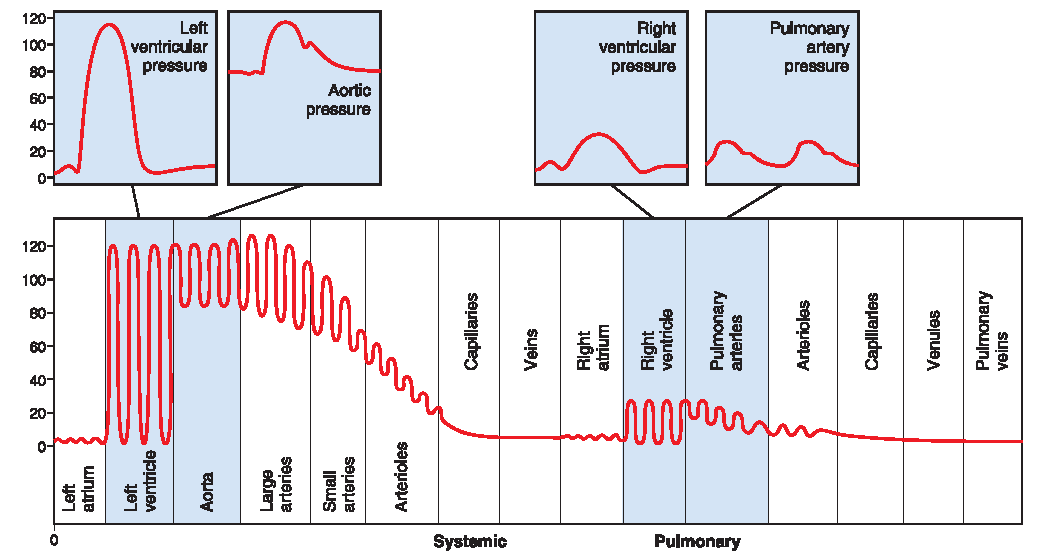
\includegraphics[width=0.9\linewidth]{ImageFiles/Fotopletismografia/PressioneSangue}
 	\caption{Pressione del sangue nelle differenti porzioni dell'apparato circolatorio quando una persona è in posizione supina.}
 	\label{fig:PressioneSangue}
\end{figure}
Mentre il sangue scorre all'interno della circolazione sistemica, la pressione media scende progressivamente fino a circa 0 mm Hg, alla terminazione della vena cava superiore e inferiore. Inoltre, anche l'andamento pulsatile tende a diminuire a livello capillare e venoso. Si noti come, nella circolazione polmonare, la pressione nelle arterie polmonari ritorni ad essere pulsatile, a causa dell'azione del ventricolo destro, ma con una pressione media di 16 mm Hg, di molto inferiore rispetto a quella dell'aorta. La bassa pressione all'interno della piccola circolazione è necessaria per permettere lo scambio gassoso a livello polmonare.

La diminuzione della pressione del flusso ematico all'interno dell'apparato circolatorio è causato dalla \textit{resistenza vascolare}, che rappresenta la frizione tra il liquido e le pareti vascolari. Il flusso attraverso i vasi sanguigni può essere quindi calcolato con la seguente formula, chiamata \textit{legge di Ohm}:
\begin{equation}
	F=\frac{\Delta P}{R}
	\label{eq:OhmsLaw}
\end{equation}
dove \textit{F} è il flusso del sangue, \textit{$\Delta$P} è il gradiente di pressione tra le due estremità di un vaso e \textit{R} è la resistenza  (\Fig~\ref{fig:FlussoSangue}).
\begin{figure}[h]
	\centering
	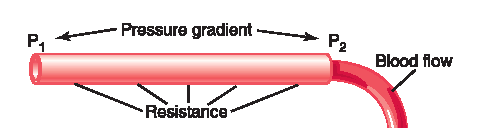
\includegraphics[width=0.7\linewidth]{ImageFiles/Fotopletismografia/FlussoSangue}
	\caption{Relazione tra pressione, resistenza e flusso ematico.P\ped{1}, pressione all'inizio del vaso, P\ped{2}, pressione all'altro capo del vaso}
	\label{fig:FlussoSangue}
\end{figure}
Il flusso indica la quantità di sangue che passa in un dato punto della circolazione in un intervallo di tempo specificato. \`E espresso in millimetri o litri al minuto. Tipicamente in un essere umano adulto il flusso è di circa 5000 ml/min.

Quando il sangue scorre con un ritmo constante all'interno di un vaso lungo e liscio, il suo flusso può essere considerato \textit{laminare}. In questo caso, la velocità del liquido ematico che si trova nel centro del vaso è maggiore rispetto a quello che si trova alle estremità, le cui particelle sono soggette alla forza d'attrito causata dal contatto con le pareti. Questo effetto è chiamato \textit{profilo parabolico della velocità del flusso del sangue} ed è mostrato nella figura \Fig~\ref{fig:FlussoParabolico}.
\begin{figure}[h]
	\centering
	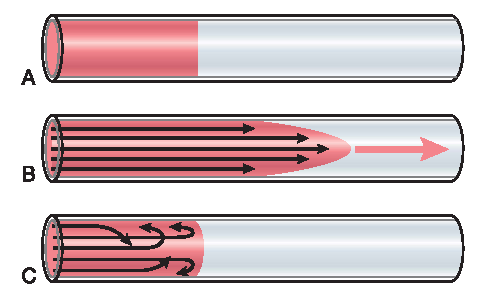
\includegraphics[width=0.7\linewidth]{ImageFiles/Fotopletismografia/FlussoParabolico}
	\caption{\textbf{A}. Due fluidi prima che il flusso inizi.\textbf{B}. Lo stesso fluido un secondo dopo l'inizio del flusso. \textbf{C}. Flusso turbolento}
	\label{fig:FlussoParabolico}
\end{figure}
Quando il ritmo diventa elevato oppure incontra una superficie ruvida o un ostacolo, il flusso non può più essere considerato laminare . Si parla quindi di \textit{flusso turbolento}, caratterizzato da un moto disordinato delle particelle del sangue che causa un aumento della resistenza.

La \textit{pressione idrostatica} del sangue rappresenta la forza esercitata dal sangue su una qualsiasi unità di area della parete di un vaso. In verità, il sangue è un liquido in movimento. Per cui, esso ha una componente dinamica, che rappresenta l'energia cinetica del sistema, da tenere in considerazione. In particolare, come si è già visto analizzando il gradiente di pressione nel circuito vascolare \todo{si dice?}, la pressione di un liquido in movimento diminuisce con la distanza percorsa, a causa dell'energia dispersa dall'attrito con le pareti del contenitore. La pressione all'interno dell'apparato circolatorio viene comunemente definita idrostatica, sebbene il sangue sia un fluido in movimento. Un'altra grandezza importante dell'emodinamica (branca della fisiologia cardiovascolare che studia il comportamento del sangue in movimento nei vasi) è la \textit{conduttanza}, che rappresenta l'attitudine di un vaso ad essere percorso dal sangue, fissato un gradiente di pressione.\`E evidente che la conduttanza è il reciproco della resistenza: 
\begin{equation}
	Conduttanza=\frac{1}{Resistenza}
	\label{eq:Conduttanza}
\end{equation}
Inoltre, la conduttanza è strettamente legata al diametro del vaso: 
\begin{equation}
	Conduttanza\propto Diametro^4
	\label{eq:ConduttanzaeDiametro}
\end{equation}
La conduttanza diminuisce al diminuire del diametro perché tutto il sangue può essere considerato a contatto con le pareti e soggetto alla resistenza. Al contrario, se il raggio aumenta, solo le particelle più esterne saranno soggette alla frizione, determinando un flusso maggiore.\todo{non mi piace molto}
Integrando le diverse velocità delle particelle del sangue in una sezione di un vaso sanguigno \todo{scrivere meglio?}, si può ricavare la seguente formula (\textit{legge di Poiseuille}):
\begin{equation}
	F\xrightarrow{}\frac{\pi\Delta P r^4}{8 \eta l}
	\label{eq:PoiseuuilleLaw}
\end{equation}
dove \textit{F} è la velocità del sangue, \textit{$\Delta$P} è il gradiente di pressione, \textit{r} è il raggio del vaso, \textit{l} la lunghezza del vaso e \textit{$\eta$} è la viscosità del sangue. Si ponga ancora l'attenzione sulla dipendenza della velocità del flusso con la quarta potenza del raggio del vaso. Quindi, il controllo del flusso del sangue può essere effettuato controllando il diametro dei vasi sanguigni. Questo permette alle arteriole di variare il flusso sanguigno nei tessuti. Al contrario, la lunghezza e la viscosità del sangue (che dipende dal rapporto tra eritrociti e plasma) possono essere considerati parametri costanti che non influenzano la pressione in modo significativo.



\todo{nell'articolo Blood Pressure Estimation from Photoplethysmogram relazione tra pressione e segnale ppg}
\pagebreak